\subsection{Executing Agent Routes in Simulation}
\note{talk about how routes can be executed in sim. env.}
In order to test the algorithms developed in this chapter in a realistic scenario, we utilised the simulation environment described in Chapter \ref{chap:HighFidelitySim}. The AirSim plugin \cite{Shah2017AirSim:Vehicles} provides a straightforward interface to be able to configure the simulation environment to run with a user specified number of UAVs, with an API to send commands to each. We successfully ran a number of tests in simulation using the User Interface to select the bounding area and grid spacing for the UAVs, which interfaced with the code which generated the routes for the UAVs. We then used the AirSim API to send the virtual UAVs to the generated waypoints on each route to gather images. The results of a simulation run showing the executed routes are shown in figure \ref{fig:VirtualPlannedRoutes}


\begin{figure}
    \centering
    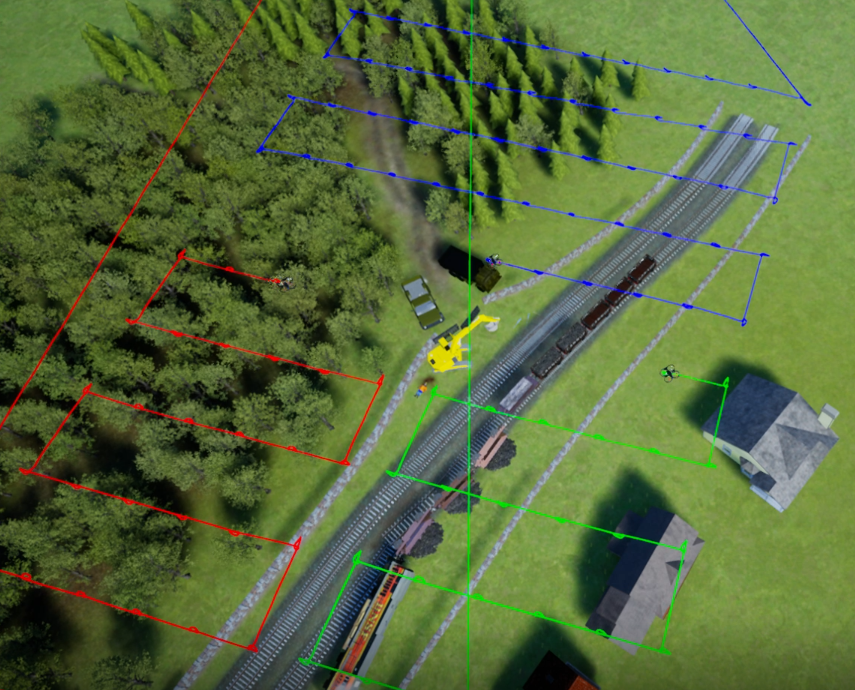
\includegraphics[width=0.6\textwidth]{Chapters/SimulationEnv/Figs/DebuggingLines/RoutesWithRAVsVisible.png}
    \caption{UAVs executing their planned routes in the simulation environment}
    \label{fig:VirtualPlannedRoutes}
\end{figure}